% Top-level Evaluation chapter. \input this from the main manuscript.
% Requires in the preamble: \usepackage{booktabs} \usepackage{amsmath} \usepackage{amssymb} \usepackage{graphicx}
% If the main document uses a different graphics path for the figures, set it before \input.
\section{Privacy Evaluation}
\label{sec:eval}

We evaluate the three privacy properties of our system---Policy Content Hiding,
Policy Indistinguishability, and Structure \& Parameter Privacy---against a passive
on-chain observer (Section~\ref{sec:eval-threat}). Each property is attacked with both a
supervised classifier and an unsupervised clustering attacker under an honest,
reproducible, multi-seed criterion (Section~\ref{sec:eval-method}). All three properties
pass under both attackers.

% Shared threat model for the three privacy experiments.
\subsection{Adversary and observables}
\label{sec:eval-threat}

We evaluate against a \emph{passive on-chain observer}: an adversary who sees every
transaction and event our approach emits, but never the plaintext policy, the witness,
or any client-side timing. This is the strongest realistic attacker for a public
blockchain---it has unrestricted, perpetual read access to the ledger.

Concretely, for each policy execution (a commit transaction followed by an access
transaction) the adversary observes the following on-chain features:
%
\begin{itemize}
  \item \textbf{Gas:} \texttt{commitGasUsed}, \texttt{accessGasUsed}.
  \item \textbf{Calldata size:} \texttt{commitCalldataLength}. \texttt{accessCalldataLength}.
  \item \textbf{Proof size:} \texttt{proofSize}.
  \item \textbf{Event logs:} \texttt{commitLogsCount}, \texttt{commitLogsSize},
    \texttt{accessLogsCount}, \texttt{accessLogsSize}.
\end{itemize}
%
By design, calldata length, proof size, and log counts/sizes are content-independent
(constant across policies), so any residual signal can only flow through the gas
features in the modeled public transcript. The effective feature set the attacker can
exploit therefore reduces to the two gas measurements (\texttt{commitGasUsed}, \texttt{accessGasUsed}); the remaining observables are retained in the pipeline but carry no policy-dependent variation. The defenses (commitment-only interface, randomized access-gas padding) target exactly this channel. We do not model other potential side channels such as block
timing, transaction ordering, mempool or broadcast patterns, or off-chain TPS
communication; compromised TPS behavior, adaptive requester probing, and off-chain side
channels remain outside this evaluation model, matching the system model in
Section~\ref{sec:problem}.

We consider three increasingly fine-grained attacker tasks, one per privacy property:
(i)~recover the policy's \emph{content} (PCH, Section~\ref{sec:eval-pch}); (ii)~tell two
\emph{semantically related} policies apart (PI, Section~\ref{sec:eval-pi}); and
(iii)~recover the policy's \emph{structure or parameter magnitude} (SPP,
Section~\ref{sec:eval-spp}). The primary attacker is supervised and label-aware; a
separate unsupervised clustering attacker provides a label-free cross-check
(Section~\ref{sec:eval-method}).

% Shared methodology: supervised attack pipeline + unsupervised clustering cross-check.
\subsection{Attack methodology}
\label{sec:eval-method}

We evaluate each privacy property with a primary supervised attack and a complementary
unsupervised cross-check. The \emph{supervised} pipeline asks whether a trained
classifier can recover a hidden label from the observables; this is the main privacy
verdict because it gives the adversary labels and therefore more power than a purely
exploratory analysis. The \emph{unsupervised} pipeline asks whether the observables
cluster along the hidden label without any supervision, providing a label-free sanity
check on the same executions.

\subsubsection{Supervised attacks}
For every task we train linear and non-linear classifiers and report the score used by
the unified verdict for that property. Each task is evaluated over \textbf{30 random
seeds} using a \textbf{policy-disjoint train/test split}: the policies used to train the
attacker never appear in the test set, so a high score cannot come from memorizing
individual policies. For each seed we run a label-permutation test and record whether
the AUC is significant at $\alpha{=}0.05$.

The honest headline metrics are the AUC, its distance from chance $|\mathrm{AUC}-0.5|$,
and the permutation $p$-value. We \emph{report} the classifier advantage over random but
do \emph{not} gate on it: on imbalanced test sets a majority-class predictor scores a
large advantage with $F_1\approx 0$, so advantage alone is unreliable. The unified
verdict (\texttt{experiments/core/multiseed\_criterion.js}) is:
%
\begin{quote}
  \textbf{PASS} iff $\mathrm{AUC}_{\text{mean}}\le 0.55$ \textbf{and} the
  significant-seed fraction is $<0.5$ (over 30 policy-disjoint seeds).
\end{quote}
%
Both legs are required: high classification power that is not statistically reproducible
across seeds (or reproducible significance with chance-level AUC) does not constitute a
leak. Subclasses whose median test size is $n<20$ are \emph{underpowered}---reported but
excluded from gating, so a tiny subclass's noise cannot decide the verdict. The result
tables report the AUC selected by the committed verdict file for each task. SPP uses the
calibrated random-forest score for its AUC leg because logistic regression
over-separates on the near-constant SPP features and yields a degenerate AUC.

\paragraph{Positive control.} To show that a chance-level AUC means \emph{no signal}
rather than a \emph{broken attack}, every supervised experiment also runs a synthetic
control: a label deterministically derived from the gas (``\texttt{gas\,>\,median}'')
pushed through the identical pipeline. The control reaches AUC $\approx 0.99$ and
$F_1\approx 0.95$, confirming the attack can detect a real channel when one exists.

\subsubsection{Unsupervised clustering attacks}
The clustering attacker drops the labels entirely and asks whether the gas features
\emph{naturally} group along the hidden property. We run K-Means (with $K$ set to the
number of classes, or $K{=}2$ for policy pairs) and DBSCAN on the on-chain gas features,
and score the recovered clusters against the true labels with the Adjusted Rand Index
(ARI) and Normalized Mutual Information (NMI). Values near $0$ mean the clusters carry no
information about the hidden label; values near $1$ mean full leakage.

PCH clusters all executions globally (no per-layer splitting), so the large-sample
ARI/NMI are read directly. For the PI pairs we additionally guard against two
small-sample failure modes.

\paragraph{Controlling sample-size confounds.} The naive PI pair construction produced
severely imbalanced pairs (one policy with $1$ execution against another with up to
$30$), where K-Means cannot cut the data and ARI/NMI $\approx 0$ is an artifact rather
than evidence of privacy. We therefore rebuild the PI pairs from policies with
$\ge 30$ executions into balanced $30$-vs-$30$ contrasts before clustering. To rule out
residual finite-sample inflation, we add a \emph{permutation baseline}: we shuffle the
pair labels $200$ times and recompute the clustering NMI, giving the NMI distribution
under zero true signal. The debiased NMI is the observed value minus this baseline, and
the empirical $p$-value is the fraction of permutations whose NMI meets or exceeds the
observed; a pair leaks only if its debiased NMI is positive \emph{and} significant
($p<0.05$).

\paragraph{Dataset.} Both attack families run on the same fixed-circuit, commitment-only,
access-gas-padded \emph{Polygon~Amoy} dataset: the supervised verdicts read
\texttt{experiments/multiseed\_results/polygonAmoy/} (numbers of record), and the
clustering reads the same executions exported to \texttt{python/data/polygonAmoy/}. The
supervised and unsupervised attacks therefore constitute two independent attack families
applied to one dataset, rather than two datasets. Per-task sample sizes vary and are
listed in the result tables (e.g.\ $2005$ DUO executions; $133$ balanced $30$-vs-$30$ PI
pairs); the PI debiasing averages each observed NMI over $20$ K-Means seeds against a
$200$-permutation baseline. Provenance for every table and figure is listed in
\texttt{paper/README.md}.

% Policy Content Hiding section body.
\subsection{Policy Content Hiding (PCH)}
\label{sec:eval-pch}

\paragraph{Property.} PCH requires that the on-chain observer cannot recover the
\emph{content} of a policy---its DUO data-use terms or the ICD-10 disease codes it
references---better than chance.

\paragraph{Scope of the labels.} We do not attack the full Data Use Ontology and its
linked ontologies. The complete DUO has 23 data-use terms, and ICD-10 has tens of
thousands of individual codes; most never appear in our generated policies, and those
that do are too rare to support a statistically powered one-vs-rest attack. We therefore
evaluate the six DUO terms that occur with enough support in the dataset (GR, DS, RS,
POA, GS, CC; smallest class $n{=}30$) and aggregate disease codes to the ten ICD-10
chapters. This is the right granularity for the privacy question---the observer cares
whether the \emph{category} of permitted use or disease leaks, not which leaf code is
used---and it is also a conservative choice: attacks on coarser, better-supported labels
are \emph{easier} than on rare leaf terms, so passing here does not understate the leak.
The defenses (commitment-only interface, gas padding) are content-agnostic and apply
identically to the terms we do not enumerate.

\paragraph{Supervised attack.} We treat each of the six DUO terms (GR, DS, RS, POA, GS,
CC) as a one-vs-rest binary recovery task and run the multi-seed pipeline of
Section~\ref{sec:eval-method}. Table~\ref{tab:pch-terms} reports the authoritative
per-term verdicts: every DUO task has $\mathrm{AUC}_{\text{mean}}\in[0.490,0.527]$ and a
significant-seed fraction of at most $13\%$, so none approaches either leg of the failure
criterion. The same pipeline applied to the ten ICD-10 chapters (one-vs-rest over the
ICD-bearing rows only; Table~\ref{tab:pch-icd10}) passes all ten. The single highest
value is ch6 at $\mathrm{AUC}_{\text{mean}}=0.573\pm0.061$ with $17\%$ significant
seeds; it clears the AUC leg ($0.573>0.55$) but not the reproducibility leg ($17\%<50\%$),
so it is a boundary case rather than a stable channel. We report such cases rather than
suppress them.

% Source of record: experiments/policy_content_hiding/results/polygonAmoy/evaluation_report.json
%   (multiseedVerdict; deterministic per-seed RNG; supersedes the older
%    multiseed_results/polygonAmoy/pch_verdict.txt batch).
% Policy Content Hiding -- supervised attack, multi-seed (30 policy-disjoint seeds).
% Criterion: FAIL iff AUC_mean > 0.55 AND significant-seed fraction >= 0.5
% (perm alpha=0.05); both legs required, else PASS.
\begin{table}[t]
  \centering
  \caption{Policy Content Hiding: per-term supervised attack over 30 policy-disjoint
    seeds. Each DUO term is a one-vs-rest binary task. \emph{\%sig} is the fraction of
    seeds whose permutation test rejects at $\alpha{=}0.05$. All six tasks pass the
    unified criterion.}
  \label{tab:pch-terms}
  \begin{tabular}{lccccc}
    \toprule
    Term & AUC (mean\,$\pm$\,std) & perm $p$ & \%sig & med $n$ & verdict \\
    \midrule
    DUO GR  & $0.497 \pm 0.024$ & $0.535$ & $0\%$  & $613$ & \checkmark \\
    DUO DS  & $0.490 \pm 0.021$ & $0.624$ & $3\%$  & $613$ & \checkmark \\
    DUO RS  & $0.527 \pm 0.019$ & $0.191$ & $13\%$ & $613$ & \checkmark \\
    DUO POA & $0.493 \pm 0.023$ & $0.579$ & $0\%$  & $613$ & \checkmark \\
    DUO GS  & $0.521 \pm 0.018$ & $0.251$ & $13\%$ & $613$ & \checkmark \\
    DUO CC  & $0.501 \pm 0.018$ & $0.479$ & $0\%$  & $613$ & \checkmark \\
    \midrule
    \multicolumn{6}{l}{Overall: \checkmark\ PASS} \\
    \bottomrule
  \end{tabular}
\end{table}

% Source of record: experiments/policy_content_hiding/results/polygonAmoy/evaluation_report.md
%   ("Multi-seed Verdict (authoritative)" table, ICD ch0-ch9 rows).
% Multi-seed (30 policy-disjoint seeds), LR+RF stronger-of-two reported.
% Criterion: FAIL iff AUC_mean > 0.55 AND significant-seed fraction >= 0.5; else PASS.
\begin{table}[t]
  \centering
  \caption{Policy Content Hiding: per-chapter ICD-10 supervised attack over 30
    policy-disjoint seeds (one-vs-rest, ICD-bearing rows only; median test $n=271$). Two
    chapters reach AUC above $0.55$ (ch4, ch6) but neither is permutation-significant
    (\%sig${}<50\%$), so all ten pass the dual criterion.}
  \label{tab:pch-icd10}
  \begin{tabular}{lcccc}
    \toprule
    Chapter & AUC (mean\,$\pm$\,std) & perm $p$ & \%sig & verdict \\
    \midrule
    ICD ch0 & $0.509 \pm 0.052$ & $0.470$ & $7\%$  & \checkmark \\
    ICD ch1 & $0.502 \pm 0.047$ & $0.510$ & $3\%$  & \checkmark \\
    ICD ch2 & $0.535 \pm 0.054$ & $0.307$ & $17\%$ & \checkmark \\
    ICD ch3 & $0.550 \pm 0.047$ & $0.236$ & $10\%$ & \checkmark \\
    ICD ch4 & $0.578 \pm 0.068$ & $0.210$ & $33\%$ & \checkmark \\
    ICD ch5 & $0.481 \pm 0.061$ & $0.543$ & $0\%$  & \checkmark \\
    ICD ch6 & $0.607 \pm 0.066$ & $0.148$ & $37\%$ & \checkmark \\
    ICD ch7 & $0.511 \pm 0.041$ & $0.431$ & $3\%$  & \checkmark \\
    ICD ch8 & $0.524 \pm 0.037$ & $0.365$ & $3\%$  & \checkmark \\
    ICD ch9 & $0.565 \pm 0.048$ & $0.257$ & $3\%$  & \checkmark \\
    \midrule
    \multicolumn{5}{l}{Overall: \checkmark\ PASS (all 10 chapters)} \\
    \bottomrule
  \end{tabular}
\end{table}

% Policy Indistinguishability section body.
\subsection{Policy Indistinguishability (PI)}
\label{sec:eval-pi}

\paragraph{Property.} PI strengthens PCH: even when two policies are \emph{semantically
related}, the observer must not tell which one was executed---formally,
$\Pr[\hat b = b]\approx \tfrac12$. We test four pair archetypes: \texttt{semantic\_%
equivalent} (identical normalized logic), \texttt{structural\_variant} (same semantics,
different execution protections), \texttt{weak\_equivalent} ($\ge 0.95$ semantic
overlap), and \texttt{controlled\_difference} (small targeted deltas; a regression
control).

\paragraph{Attacker levels.} The distinguisher's task is to decide, from the on-chain
features of an execution, which policy of the pair produced it. We try three attackers of
increasing strength: \emph{Level~I} trains a classifier on the features of a single
execution; \emph{Level~II} compares the feature \emph{difference} between the two
policies' executions (a paired attacker); and \emph{Level~III} runs two-sample
statistical tests (Kolmogorov--Smirnov and Maximum Mean Discrepancy) directly on the two
feature distributions. A pair is indistinguishable only if all three stay at chance.

\paragraph{Results.} Our primary attacker is Level~I, evaluated over 30 policy-disjoint
seeds (Table~\ref{tab:pi-pairs}): the overall AUC is $0.480\pm0.042$ with $0\%$ of seeds
significant, and every archetype that has enough test data passes. Only
\texttt{weak\_equivalent} is set aside---its median test set is $n=9$, below the
power threshold of Section~\ref{sec:eval-method}, so it is reported but not gated. The
stronger Level~II and Level~III attackers, measured on a single split as a diagnostic,
are likewise at chance (Level~II overall AUC $0.500$; Level~III MMD $\le 0.05$ with
non-significant KS), so no attacker separates the pairs.

\paragraph{Why multi-seed matters.} At three seeds the \texttt{structural\_variant}
archetype read AUC $0.69$ with $100\%$ of seeds significant---enough to look like a
leak---but at 30 seeds it regressed to $0.541\pm0.095$ with only $40\%$ significant,
revealing the spike as a small-sample fluke. The final 30-seed verdict
(Table~\ref{tab:pi-pairs}, AUC $0.535\pm0.088$, $20\%$ significant) confirms the pass.
This is precisely the failure mode the multi-seed criterion of
Section~\ref{sec:eval-method} is designed to reject.

\paragraph{Clustering attack.} On balanced $30$-vs-$30$ pairs (133 pairs, after the
sample-size correction of Section~\ref{sec:eval-method}) K-Means recovers no structure:
mean ARI $0.0015$, mean observed NMI $0.0136$, mean debiased NMI $0.0012$
(Table~\ref{tab:clustering-summary}). Only $6/133$ pairs cross the per-pair significance
threshold---consistent with the $\approx 5\%$ false-positive rate expected by chance at
$\alpha{=}0.05$---so PI holds under the unsupervised attacker as well.

% Source of record: experiments/multiseed_results/polygonAmoy/pi_verdict.txt
% Policy Indistinguishability — supervised distinguisher, multi-seed (30 policy-disjoint seeds).
% Criterion: AUC_mean <= 0.55 AND significant-seed fraction < 0.5 (perm alpha=0.05).
% weak_equivalent is underpowered (median test n=9 < 20): reported, excluded from gating.
\begin{table}[t]
  \centering
  \caption{Policy Indistinguishability: single-sample distinguisher (Level~I) over 30
    policy-disjoint seeds, by policy-pair archetype. A negative advantage means the
    attacker does worse than chance. \texttt{weak\_equivalent} has median test $n{=}9{<}20$
    and is reported but excluded from the verdict (underpowered).}
  \label{tab:pi-pairs}
  \begin{tabular}{lcccccc}
    \toprule
    Pair archetype & AUC (mean\,$\pm$\,std) & adv (mean\,$\pm$\,std) & perm $p$ & \%sig & med $n$ & verdict \\
    \midrule
    overall               & $0.480 \pm 0.042$ & $-0.059 \pm 0.045$ & $0.627$ & $0\%$  & $369$   & \checkmark \\
    semantic\_equivalent  & $0.410 \pm 0.057$ & $-0.121 \pm 0.069$ & $0.811$ & $0\%$  & $57$    & \checkmark \\
    structural\_variant   & $0.535 \pm 0.088$ & $-0.033 \pm 0.092$ & $0.346$ & $20\%$ & $118.5$ & \checkmark \\
    weak\_equivalent      & $0.443 \pm 0.152$ & $-0.196 \pm 0.128$ & $0.667$ & $0\%$  & $9$     & --\,(underpwr.) \\
    controlled\_difference& $0.512 \pm 0.051$ & $-0.051 \pm 0.075$ & $0.447$ & $7\%$  & $126$   & \checkmark \\
    \midrule
    \multicolumn{7}{l}{Overall: \checkmark\ PASS} \\
    \bottomrule
  \end{tabular}
\end{table}

% Structure & Parameter Privacy section body.
\subsection{Structure \& Parameter Privacy (SPP)}
\label{sec:eval-spp}

\paragraph{Property.} SPP requires that neither the \emph{shape} of a policy (logical
structure, nesting depth, predicate coverage) nor the \emph{magnitude} of its parameters
(set sizes, range widths) leaks to the observer. We organize the test along three
annotation axes---structure type, predicate combination, and parameter magnitude---and
attack each pair of buckets within an axis.

\paragraph{Supervised attack.} Table~\ref{tab:spp-contrasts} reports all 18 pairwise
contrasts over 30 policy-disjoint seeds. AUC is the calibrated random-forest score, since
logistic regression over-separates on the near-constant SPP features. Every contrast has
$\mathrm{AUC}_{\text{mean}}\in[0.43,0.52]$ and a significant-seed fraction at or below
$27\%$, so all 18 pass and SPP passes overall. The no-predicate (\texttt{none}$_{\text{pred}}$)
contrasts illustrate why we gate on AUC rather than advantage: their single-split
logistic-regression advantage looks large ($0.42$--$0.48$), but this is the
majority-class artifact described in Section~\ref{sec:eval-method}---a near-constant
predictor scoring high advantage on an imbalanced split without genuine separation---and
the AUC-plus-permutation criterion correctly reads these as chance.

\paragraph{Positive control.} The synthetic \texttt{gas\,>\,median} control reaches AUC
$1.000\pm0.001$ and $F_1=1.00$ through the same pipeline, validating that the
chance-level scores on real structure/parameter labels reflect the absence of signal.

\paragraph{Clustering attack.} Unsupervised K-Means over the gas features recovers none
of the four structural targets (Table~\ref{tab:clustering-summary}): \texttt{logicStructure}
ARI $-0.0015$/NMI $0.0011$, \texttt{nestingDepth} $-0.0002$/$0.0018$,
\texttt{predicateCount} $-0.0008$/$0.0015$, and \texttt{setSize} $-0.0013$/$0.0019$---all
indistinguishable from random partitions. Structure and parameters are hidden under both
the supervised and the unsupervised attacker.

% Source of record: experiments/structure_and_parameter_privacy/results/polygonAmoy/report.json
%   (multiseedVerdict, deterministic per-seed RNG; this is the current of-record run.
%    The older experiments/multiseed_results/polygonAmoy/spp_verdict.txt batch is superseded.)
% Structure & Parameter Privacy — supervised attack, multi-seed (30 policy-disjoint seeds).
% AUC uses random forest (LR over-separates on near-constant features).
% Criterion: AUC_mean <= 0.55 AND significant-seed fraction < 0.5 (perm alpha=0.05).
% table* spans both columns (the 6-column rows with two mean+-std columns overflow a single column).
\begin{table*}[t]
  \centering
  \caption{Structure \& Parameter Privacy: 18 pairwise contrasts across three annotation
    axes, each over 30 policy-disjoint seeds. AUC is the calibrated random-forest score.
    Every contrast satisfies AUC$_{\text{mean}}\le 0.55$ \emph{and} \%sig${}<50\%$.}
  \label{tab:spp-contrasts}
  \begin{tabular}{lccccc}
    \toprule
    Contrast & AUC (mean\,$\pm$\,std) & AUC gap (mean\,$\pm$\,std) & perm $p$ & \%sig & med $n$ \\
    \midrule
    \multicolumn{6}{l}{\textit{structureType}} \\
    and\_only / or\_only              & $0.493 \pm 0.041$ & $0.030 \pm 0.029$ & $0.532$ & $3\%$  & $185$ \\
    and\_only / negation\_heavy       & $0.507 \pm 0.045$ & $0.034 \pm 0.030$ & $0.432$ & $7\%$  & $173$ \\
    and\_only / and\_or\_mixed        & $0.500 \pm 0.037$ & $0.031 \pm 0.019$ & $0.499$ & $0\%$  & $141$ \\
    or\_only / negation\_heavy        & $0.530 \pm 0.033$ & $0.034 \pm 0.029$ & $0.295$ & $20\%$ & $199$ \\
    or\_only / and\_or\_mixed         & $0.489 \pm 0.039$ & $0.034 \pm 0.021$ & $0.573$ & $0\%$  & $171$ \\
    negation\_heavy / and\_or\_mixed  & $0.516 \pm 0.036$ & $0.034 \pm 0.020$ & $0.392$ & $0\%$  & $154$ \\
    \midrule
    \multicolumn{6}{l}{\textit{predicateCombo}} \\
    none / single   & $0.461 \pm 0.192$ & $0.171 \pm 0.095$ & $0.542$ & $4\%$  & $74$  \\
    none / few      & $0.499 \pm 0.202$ & $0.157 \pm 0.127$ & $0.508$ & $7\%$  & $215$ \\
    none / many     & $0.476 \pm 0.211$ & $0.167 \pm 0.132$ & $0.508$ & $0\%$  & $59$  \\
    single / few    & $0.496 \pm 0.033$ & $0.027 \pm 0.019$ & $0.533$ & $0\%$  & $284$ \\
    single / many   & $0.490 \pm 0.045$ & $0.035 \pm 0.031$ & $0.563$ & $3\%$  & $128$ \\
    few / many      & $0.478 \pm 0.035$ & $0.033 \pm 0.026$ & $0.643$ & $0\%$  & $268$ \\
    \midrule
    \multicolumn{6}{l}{\textit{paramType}} \\
    none / small    & $0.444 \pm 0.205$ & $0.159 \pm 0.140$ & $0.571$ & $3\%$  & $66$  \\
    none / medium   & $0.507 \pm 0.262$ & $0.212 \pm 0.154$ & $0.482$ & $15\%$ & $203$ \\
    none / large    & $0.421 \pm 0.203$ & $0.176 \pm 0.128$ & $0.606$ & $4\%$  & $77$  \\
    small / medium  & $0.510 \pm 0.038$ & $0.032 \pm 0.022$ & $0.423$ & $3\%$  & $263$ \\
    small / large   & $0.527 \pm 0.036$ & $0.037 \pm 0.027$ & $0.336$ & $3\%$  & $139$ \\
    medium / large  & $0.499 \pm 0.031$ & $0.025 \pm 0.017$ & $0.510$ & $3\%$  & $277$ \\
    \midrule
    \multicolumn{6}{l}{Overall: \checkmark\ PASS (all 18 contrasts)} \\
    \bottomrule
  \end{tabular}
\end{table*}

% Cross-property unsupervised clustering section (consolidated view + PI rebalancing).
% Figures are tracked under figures/ (copied from the gitignored python/results/ tree).
% main.tex sets \graphicspath{{figures/}{./}}; this local \graphicspath is a fallback so
% the chapter also resolves figures when compiled on its own (e.g. via _smoke.tex).
\graphicspath{{figures/}{./}}
\subsection{Unsupervised clustering: a label-free cross-check}
\label{sec:eval-clustering}

The supervised attacks (Sections~\ref{sec:eval-pch}--\ref{sec:eval-spp}) assume an
adversary who can train on labeled executions. A weaker but assumption-free attacker
simply asks whether the on-chain gas features \emph{cluster} along the hidden property
with no supervision at all. Table~\ref{tab:clustering-summary} consolidates this attack
across all three properties: K-Means recovers essentially nothing, with ARI and NMI
within $\pm 0.02$ of zero for every DUO, PI, and SPP target. NMI values are interpreted
against the null finite-sample simulation in Section~\ref{sec:eval-nmi-sensitivity}.
The unsupervised attacker
agrees with the supervised verdict---privacy holds---as a second, label-free attack family
on the same dataset (Figure~\ref{fig:clust-summary}).

\begin{figure}[t]
  \centering
  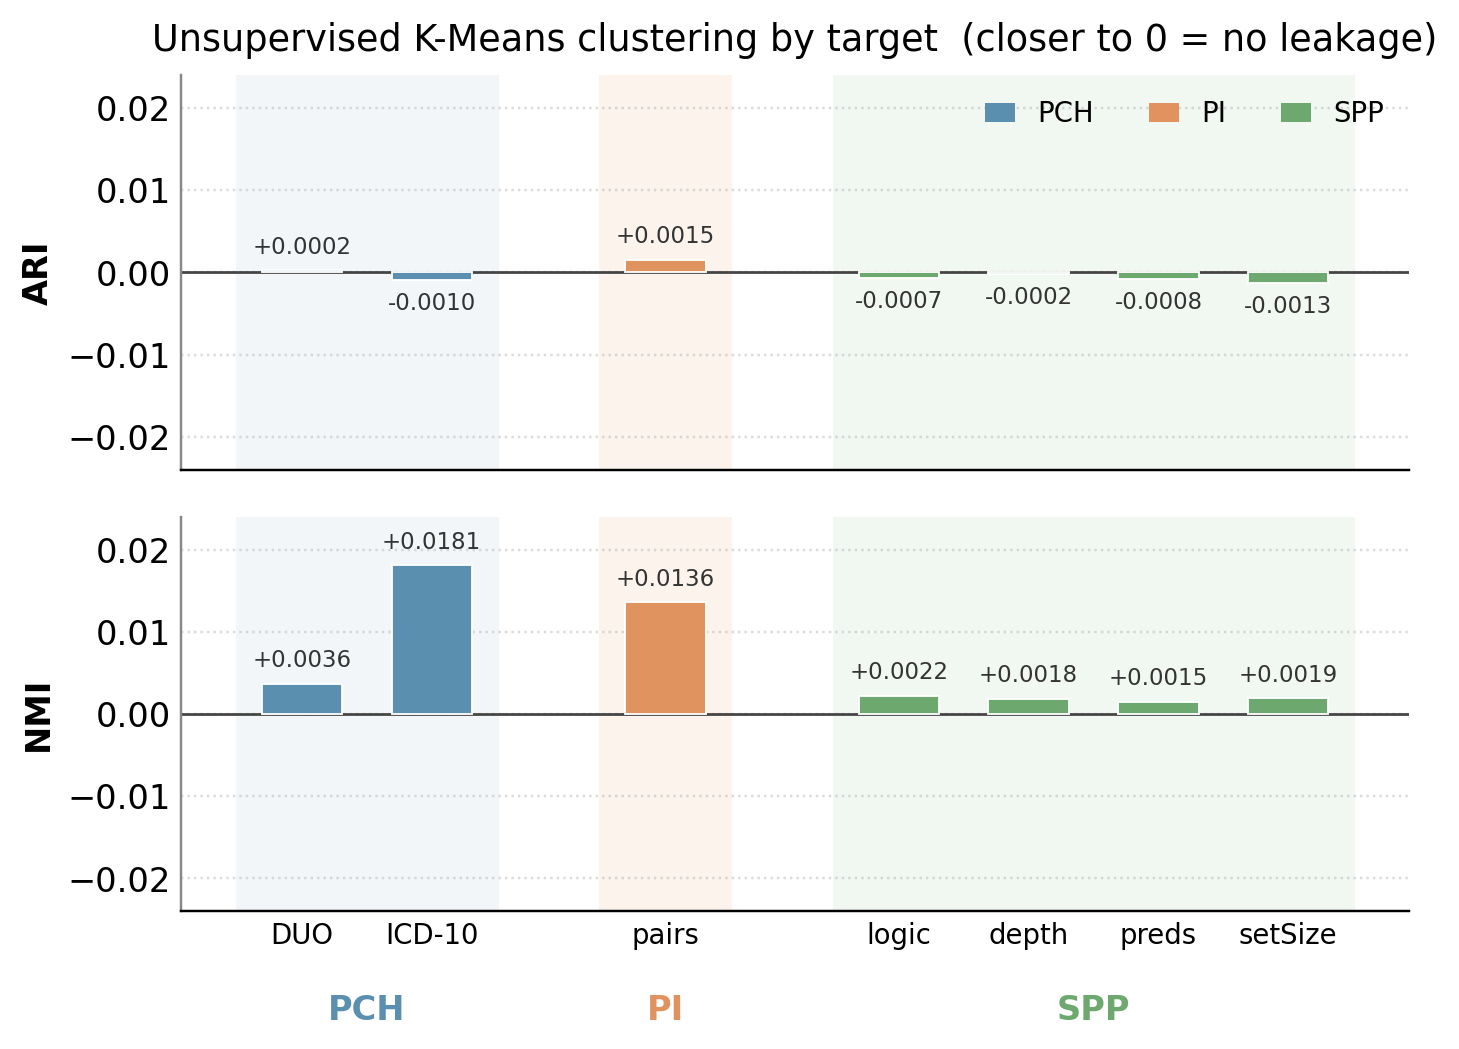
\includegraphics[width=\linewidth]{clustering_summary_unified.png}
  \caption{Unsupervised K-Means clustering across all three properties on a common
    axis: ARI (top) and NMI (bottom) for every PCH, PI, and SPP target. Every bar sits
    at the zero line---the natural gas clusters carry no information about the hidden
    label. SPP targets are abbreviated (logic: \texttt{logicStructure}; depth:
    \texttt{nestingDepth}; preds: \texttt{predicateCount}; setSize: \texttt{setSize}).
    NMI is read against the null finite-sample simulation in
    Section~\ref{sec:eval-nmi-sensitivity}.}
  \label{fig:clust-summary}
\end{figure}

\paragraph{Removing sample-size confounds.} The clustering inputs are constructed to
avoid degenerate measurements. The naive PI pairs were severely imbalanced (executions in
a $1{:}30$ ratio), under which K-Means trivially fails and a low ARI/NMI would be
meaningless. We rebuild the pairs into balanced $30$-vs-$30$ contrasts, and guard the
result with a permutation baseline---NMI under shuffled labels, where no true signal can
exist---reporting the debiased NMI (observed minus baseline) and its empirical $p$-value.
The conclusion is unchanged (Section~\ref{sec:eval-pi}): the indistinguishability is a
property of the protocol, not of a degenerate measurement. The ablation in
Section~\ref{sec:eval-ablation} supplies the positive control: clustering significance
appears on the un-padded gas transcript and disappears after normalization.

% Sources of record:
%   PCH-DUO:   python/results/pch_clustering_analysis/pch_global_duo_clustering.csv
%              (global, all 2005 executions, no layering)
%   PCH-ICD10: python/results/pch_clustering_analysis/pch_global_icd10_clustering.csv
%              (global, all 920 ICD-bearing executions, no layering)
%   PI:        python/results/pi_clustering_analysis/pi_balanced_debiased.csv
%              (133 balanced 30v30 pairs; observed means)
%   SPP:       python/results/spp_clustering_analysis/spp_clustering_summary.csv
% Dataset: Polygon Amoy, exported to python/data/polygonAmoy/ (same executions as the
%   supervised verdicts). See paper/README.md provenance.
\begin{table}[t]
  \centering
  \caption{Unsupervised clustering attack (K-Means, $K$=number of classes / $K{=}2$ for
    pairs) on the on-chain gas features. ARI and NMI near $0$ mean the natural gas
    clusters carry no information about the hidden label. PCH clusters all executions
    globally (no layering).}
  \label{tab:clustering-summary}
  \footnotesize
  \setlength{\tabcolsep}{4pt}
  \begin{tabular}{@{}llcccc@{}}
    \toprule
    Property & Target & $n$ & \#cls. & ARI & NMI \\
    \midrule
    PCH & DUO terms                & $2005$ & $6$  & $0.0002$  & $0.0036$ \\
    PCH & ICD-10 chapters          & $920$  & $10$ & $-0.0010$ & $0.0181$ \\
    PI  & policy pairs ($30$v$30$) & $133$  & $2$  & $0.0015$  & $0.0136$ \\
    SPP & logicStructure           & $1141$ & $4$  & $-0.0007$ & $0.0022$ \\
    SPP & nestingDepth             & $1141$ & $4$  & $-0.0002$ & $0.0018$ \\
    SPP & predicateCount           & $1141$ & $4$  & $-0.0008$ & $0.0015$ \\
    SPP & setSize                  & $1141$ & $4$  & $-0.0013$ & $0.0019$ \\
    \bottomrule
  \end{tabular}
\end{table}

